% This version of CVPR template is provided by Ming-Ming Cheng.
% Please leave an issue if you found a bug:
% https://github.com/MCG-NKU/CVPR_Template.

%\documentclass[review]{cvpr}
\documentclass[final]{cvpr}

\usepackage{times}
\usepackage{epsfig}
\usepackage{graphicx}
\usepackage{amsmath}
\usepackage{amssymb}
\usepackage{subfigure}
\usepackage{xcolor}
\usepackage{appendix}
% Include other packages here, before hyperref.

% If you comment hyperref and then uncomment it, you should delete
% egpaper.aux before re-running latex.  (Or just hit 'q' on the first latex
% run, let it finish, and you should be clear).
\usepackage[pagebackref=true,breaklinks=true,colorlinks,bookmarks=false]{hyperref}
\usepackage{listings}

\def\cvprPaperID{****} % *** Enter the CVPR Paper ID here
\def\confYear{CVPR 2021}
%\setcounter{page}{4321} % For final version only


\begin{document}

%%%%%%%%% TITLE
\title{MLRSeg:Multi-Layer Range Point Cloud Semantic Segmentation Based on U-Net }

\author{Delin Feng\\
2020233246\\
{\tt\small fengdl@shanghaitech.edu.cn}
% For a paper whose authors are all at the same institution,
% omit the following lines up until the closing ``}''.
% Additional authors and addresses can be added with ``\and'',
% just like the second author.
% To save space, use either the email address or home page, not both
\and
Longtian Qiu\\
2018533107\\
{\tt\small qiult@shanghaitech.edu.cn}
\and
Qianjing Shi\\
2018533194\\
{\tt\small shiqj@shanghaitech.edu.cn}
}

\maketitle


%%%%%%%%% ABSTRACT
\begin{abstract}
To date, as development in 5G network and AI or autonomous driving, there has been a surge of interest in 3D point cloud semantic segmentation. Generally speaking, there are three paradigms for point cloud semantic segmentation: projection-based, discretization(voxel) based, and point-based methods. Each of these three methods has its advantages, while, how to solve the lack of small object information in the scene is still a puzzle. In this project,  we propose a multi-layer range network for semantic segmention based on U-Net, to solve the problem of missing detailed structure and pose after projection or down-sampling and improve the efficiency and accuracy of the algorithm. Inspired by the voxel structure of Cylinder3D, multilayer processing of the original point cloud data is carried out on the basis of projection-based method, so that it has the advantages similar to voxel.  We verify our algorithm via SemanticKITTI dataset and compare results with state of the art methods to evaluate the performance of the algorithm. We also create our own(ShanghaiTech campus) dataset for experiments to verify the efficiency and accuracy of the algorithm.
\end{abstract}

%%%%%%%%% BODY TEXT
\section{Introduction}
Since deep-learning, machine learning, and computer visions attracts more and more interest, point cloud segmentation (PCS) and 3D point cloud semantic segmentation (PCSS) \cite{2014Features}are popular right now, which is a fundamental and essential capability for real-time intelligent systems like autonomous driving and augmented reality. In large scale 3D point clouds, more semantic information can be provided through efficient semantic segmentation. 
\begin{figure}[h]
	\centering
	\subfigure[Ground truth segmentation]{
		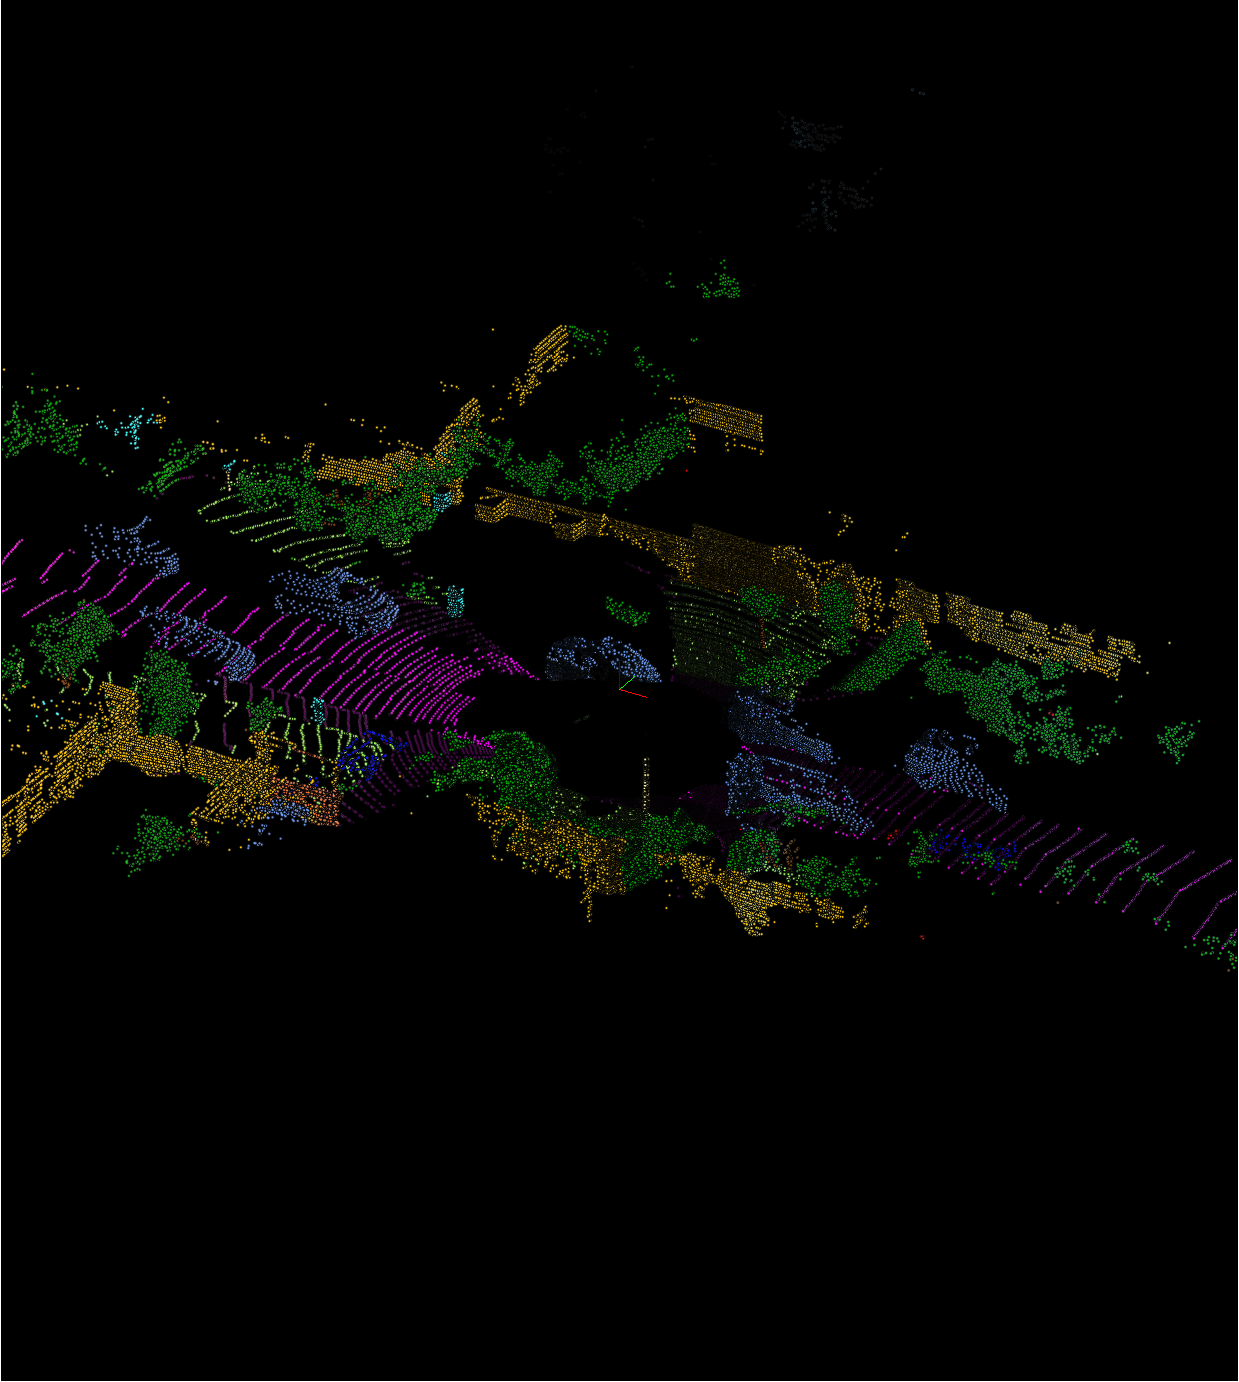
\includegraphics[width = 0.2\textwidth,height=1.5in]{latex/gt.png}
	}
	\quad
	\subfigure[Predicted segmentation]{
		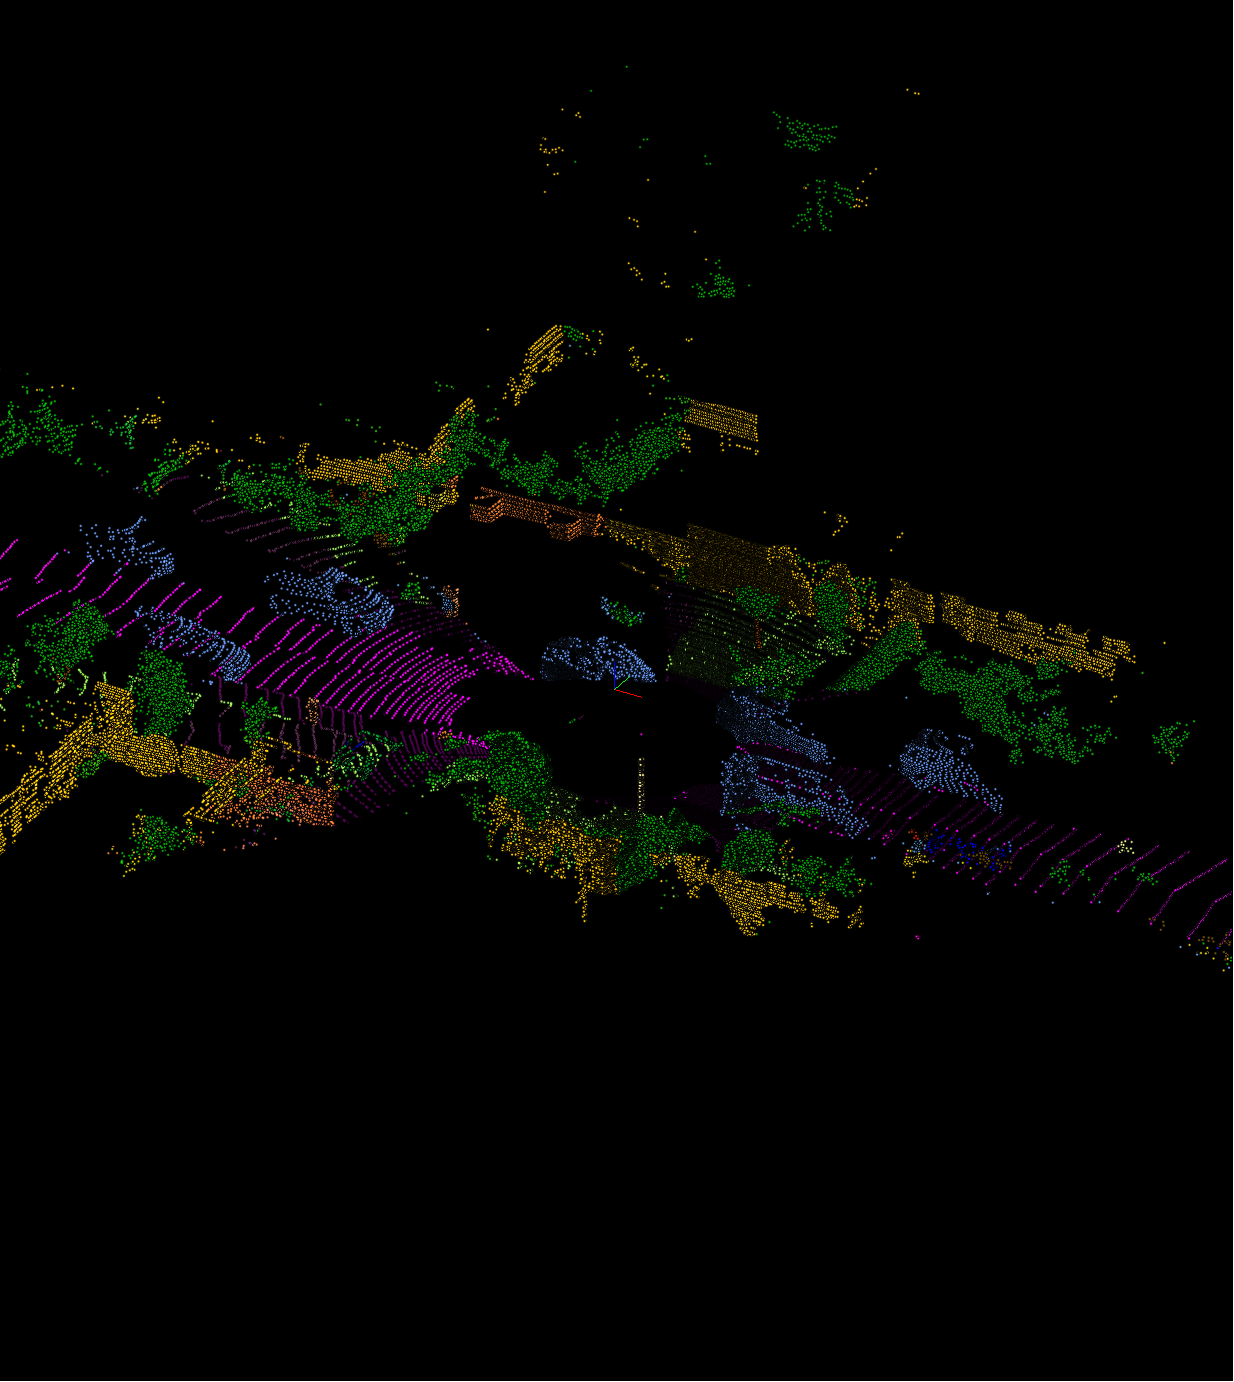
\includegraphics[width = 0.2\textwidth,height=1.5in]{latex/our.png}
	}
	\quad
	\caption{An example of MLRSeg segmentation results. Our predicted  result  is  on  the  right  and  the  ground  truth  is  on the left. }
\end{figure}
	\label{fig:per}
People have found that deep learning’s effectiveness for point cloud perception tasks. We are recently witnessing an increasing availability of not interpreted point clouds and 3D models, often shared online using point-based rendering solutions (e.g. PoTree) of mesh-based portals (e.g. Sketchfab). When it comes to point clouds, innovative methods are needed more and more for the analysis and treatment of these data and for their classification, which we finally want to exploit in-depth the informative value of these surveys and representations. The simplest and powerful collection of elementary geometrical primitives are 3D point clouds, but at the same time  able to represent shape, size, position and orientation of objects in space\cite{Zhang2018}. This information may be augmented with additional contents obtained from other sensors or sources, such as colours, multi-spectral or thermal information, etc. For a successful exploitation of point clouds and to better understand them, we must first proceed with segmentation and classification procedures. The former refers to group points in subsets (normally called segments) characterized by having one or more characteristics in common (geometric, radiometric, etc.) whereas classification means the definition and assignment of points to specific classes (“labels”) according to different criteria. Due to the complexity and variety of point clouds caused by irregular sampling, varying density, different types of objects, etc., point cloud classification and segmentation are very active research topics\cite{Weinmann2016Reconstruction}. There are multiple research studies related to these two topics, many driven by specific needs provided by the field of application (building modeling, Heritage documentation and preservation, robotics, etc.). Most of the segmentation algorithms are tailored to work with a 2.5D surface model assumption, coming for example from a LiDAR-based survey\cite{2017A}. Many algorithms require a fine-tuning of different parameters depending upon the nature of data and applications. Supervised methods are the majority with a training phase mandatory and fundamental to guide the successive machine learning classification solution. Some of the techniques developed for segmenting point clouds generated from airborne laser scanning can be applied or easily adapted to terrestrial point clouds. The results are generally affected by noise and density of the cloud as well as by the quality of the training data\cite{2017A}.
Conventionally, researchers change the point cloud into voxel grids, then process them using 3D volumetric convolutions. It will produce information loss due to low resolutions during voxelization which means many points, if they lie in the same grid, will be merged together. So it is essential to find a high-resolution representation to preserve the fine details in the input data so as to keep it less blur. 
But it is true that both memory requirement and computational cost increase cubically with voxel resolution. Recently, another models stream try to process the input point clouds directly. Due to the sparse representation, these point-based models need much lower GPU memory which is not as much as voxel-based models. But the fact is omitted that the random memory access is not as efficient other methods. For semantic segmentation, projection-based methods can perform more quickly, but the discretization errors and fuzzification of CNN output controls the limit of them. 

Semantic segmentation is very basic in graph or imaging processing challenge, which is a method which associates pixels with semantic labels. As more and needs in 3D scenes, PCSS begins to take the responsibility, which plays the role in 3D form of it.  Semantic segmentation can use 2D image's regular distributed pixels while through PCSS, it can use irregular or regular distributed points in a 3D place. The sensors get point cloud directly and it measures the distance. Point cloud can be also generated from multi or stereo imagery view\cite{2014Features}.


We find that projection-based methods include contextual information, but lack 3D structural details. The voxel-based method includes the 3D structure of the point cloud, but requires high resolution and a large memory footprint.  Therefore, we want to integrate the advantages of the two methods and construct rich features through multi-dimensional information to achieve a better segmentation effect. Motivated by this, We process point clouds based on spherical coordinate projection to obtain range images, to fuse the features of projection-based and voxel-based methods, we design a multi-layer range image model. Meanwhile, in order to improve the recognition effect of small objects, we propose a U-Net-based convolutional neural network as the backbone of our algorithm. Since there is less open source data for point cloud semantic segmentation, we collect data from the ShanghaiTech campus for experiments.  We verify our algorithm via SemanticKITTI\cite{behley2019iccv}\cite{geiger2012cvpr} dataset and Shanghaitech Campus dataset and compare results with state of the art methods to evaluate the performance of the algorithm.
Our key contribution can be concluded as follows: 
\begin{enumerate}
\item Design a multi-layer range images model which integrates projection-based and voxel-based frameworks. 
\item Propose a convolutional neural network for semantic segmentation Based on U-Net. 
\item The experiments on validation set of SemanticKITTI dataset, our methods shows better performance on some small objects and long-distance objects.
\item The point cloud data of ShanghaiTech campus is collected as our own data set, which qualitatively illustrates the feasibility of our algorithm.
\end{enumerate}

%-------------------------------------------------------------------------
\section{Related Work(State of the Art)}
For point-cloud segmentation, papers are based on two categories, one is about small-scale point clouds, the other is about large scale point clouds. In research of small scale point cloud segmentation like indoor scene understanding or object part parsing, researchers often use  DGCNN\cite{50} PointNet\cite{35}\cite{36}. Another method, Deep-KdNet\cite{20}, groups neighbor point to extend the hierarchical architecture of PointNet++\cite{36}.

Previous approaches about point clouds recognition\cite{1}\cite{2} mainly rely on complicated hand-crafted features, such as surface normal or generated descriptors, and hard thresh old decision rules based on a clustering algorithm. These approaches have two problems: (1) hand-crafted features cost much time and the results by hard threshold decision are not suitable for productions; (2) they can not recognize the pixel level object category as the same as the semantic segmentation, which makes it difficult to apply to some autonomous driving tasks\cite{2018PointSeg}.

Here are some recent approaches for deep learning in the 3D point cloud data, semantic segmentation network structure, semantic segmentation tasks and bounding box detection tasks\cite{2018PointSeg}. 

Obtaining annotations, especially point-wise or pixel-wise annotations for computer vision tasks is usually very difficult. As a consequence, synthetic data sets have seen growing interest. In the autonomous driving community, the video game Grand Theft Auto has been used to retrieve data for object detection and segmentation\cite{019}\cite{020}\cite{4}.

CNN\cite{6} approaches consider LiDAR point clouds in either two or three dimensions. Work with two-dimensional data considers raw images with projections of LiDAR point clouds top-down\cite{014} or from a number of other views\cite{015}. Other work considers three-dimensional data itself, discretizing the space into voxels and engineering features such as disparity, mean, and saturation\cite{016}. Regardless of data preparation, deep learning methods consider end to end models that leverage 2D convolutional\cite{017} or 3D convolutional\cite{018} neural networks\cite{4}. 

FCN\cite{6} was the pioneering method for semantic segmentation based on deep learning. It replaced the last fullyconnected layers in the classification task with convolution layers. Recent approaches like DeeplabV3\cite{7} used a dilated convolutional layer\cite{8} and the conditional random field (CRF)\cite{9} to improve the prediction accuracy. SegNet\cite{10} used an encoder-decoder architecture to fuse the feature maps from the deep layer with spatial information from lower layers. Other approaches like ICnet\cite{11}, RefifineNet\cite{12} took multi-scale features into consideration and combined image features from multiple refined paths. Among those methods, Networks like Deeplabv3 and FCN were compelled to increase the performance. SegNet and ICNet are able to achieve real-time performance. Although, they have a big improvement in speed or accuracy, these methods still have some influence on the other side\cite{4}. 

3D data has sufficient features and attracts much research attention. With the rapidly developing of deep learning, many methods apply convolutional neural networks (CNN) on the 3D point cloud data directly. 3DFCN\cite{13} and VoxelNet\cite{14} used a 3D-CNN\cite{15} to extract features from width, height and depth simultaneously. MV3D\cite{16} fused multi-perception from a bird’s-eye view, a front view and a camera view to obtain a more robust feature representation. In addition, some works\cite{17} considered the representation of three-dimensional data itself and divided it into voxels to undertake features such as intensity, distance, local mean and disparity. Although all of the above methods have achieved a good accuracy, they still cost too much time in computation which limited their applications in real-time tasks\cite{2018PointSeg}.

Previous works proposed several different algorithms for plane extractions from 3D point clouds, such as RANSAC based (random sample consensus)\cite{18} methods and region grow-based methods\cite{19}. However, RANSAC requires much computation on random plane model selection. Region grow-based methods, depending on the manually designed threshold, are not adaptive. Other traditional approaches based on clustering algorithms just realized the segmentation work but not pixel-wise region classifications\cite{2018PointSeg}. 

Recently, researchers started focusing on the semantic segmentation of 3D LiDAR point cloud data. PointNet\cite{35} explored a deep learning architecture to do the 3D classification and segmentation on raw 3D data. However, it only works well in indoor. Also Dube\cite{21} explored an incremental segmentation algorithm, based on region growing, to improve the 3D task performance. However, real-time performance is still challenging. SqueezeSeg\cite{4} is similar with our task which used the SqueezeNet\cite{3} as the backbone and performed compatible results. However, it only referred the CRF to improve the performance in the predicted 2D spherical masks, which could lose location information in the 3D space. Without considering the 3D constraints in the original point cloud, the results of SqueezeSeg is extremely limited by this CRF post-process\cite{2018PointSeg}. 

\section{Method Description}
\subsection{Point Cloud Transformation}
\begin{figure}[t]
\begin{center}
% \fbox{\rule{0pt}{2in} \rule{0.9\linewidth}{0pt}}
   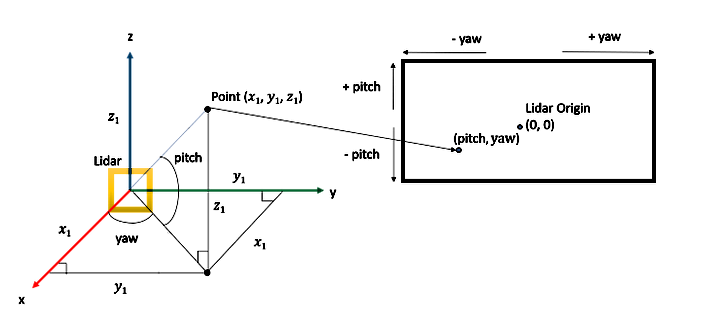
\includegraphics[width=1\linewidth]{proj.png}
\end{center}
   \caption{Explanation of spherical projection principle}
\label{fig:proj}
\end{figure}
Wu proposed an spherical projection method named SqueezeSeg\cite{4} to convert the three-dimensional point cloud in the Cartesian coordinate system into the two-dimensional range image , so that the projection-based method is widely used in the perception task of the three-dimensional point cloud. The pixel coordinates of the range image can be expressed by using a spherical coordinate system. Looking at Figure \ref{fig:proj}, we can see that if positive direction of $x$ axis is the front view of the LiDAR, then each point cloud of the scan will form an inclination angle. The image is formed by projecting a hollow cylinder onto the $zy$ plane. Since the origin is located at the center of the image, these yaw and pitch values constitute each pixel position of the projected image as Equation \ref{equ:proj}. 
\begin{equation}\label{equ:proj}
 \begin{split}
   \theta =\arcsin \frac{z}{\sqrt{x^2+y^2+z^2}}, \tilde{\theta}=[\theta / \triangle \theta ].\\
\varphi =\arcsin \frac{y}{\sqrt{x^2+y^2}}, \tilde{\varphi}=[\varphi / \triangle \varphi ].
  \end{split}
\end{equation}
$\theta$ and $\varphi$ are pitch and yaw angles as shown in Figure \ref{fig:proj}. $\triangle \theta$ and $\triangle \varphi$ are resolutions for discretization and $\tilde{\theta}$ and $\tilde{\varphi}$ denotes the position of a point on a 2D spherical grid.  The pitch angle $\theta \in [FOV_{Up}, FOV_{Down}]$, where $FOV$ is the filed of view, and yaw angle $\varphi \in [-\pi, \pi]$.
\begin{figure}[b]
\begin{center}
% \fbox{\rule{0pt}{2in} \rule{0.9\linewidth}{0pt}}
   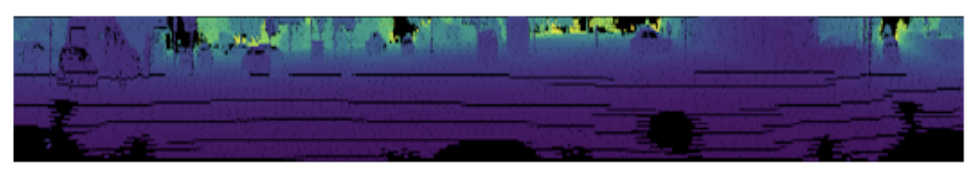
\includegraphics[width=1\linewidth]{projex.png}
\end{center}
   \caption{An example of range image}
\label{fig:projex}
\end{figure}
This procedur results in a list of $(u,v)$ tuples containing a pair of image coordinates for each point cloud. Using these  indexes, we extract for each point cloud, its ranger, its $x$,$y$ and $z$ coordinates, and its remission, and we store them in the image, creating a $[5,H,W]$ tensor, where $H,W$ are range image's height and width. Because of the de-skewing of the scan,the assignment of each points to its corresponding $(u,v)$ is done in a descending range order, to ensure that all points rendered in the image are in the current field of view of the sensor. We furthermore save this list of $(U,V)$ pairs to gather and clean the semantics of the resulting point cloud, as we describe in Section 4. We get range images as shown in Figure \ref{fig:projex}.



\begin{figure}[htbp]
\begin{center}
% \fbox{\rule{0pt}{2in} \rule{0.9\linewidth}{0pt}}
   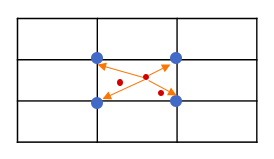
\includegraphics[width=0.6\linewidth]{latex/round.png}
\end{center}
   \caption{Representation of $\theta$ and $\varphi$'s discretization}
\label{fig:qua}
\end{figure}

In this project, we also considered the discretization of $\theta$ and $\varphi$.  Due to the nature of spherical projection, points on similar rays are projected onto the image, as shown in Figure \ref{fig:qua}, they will be in a grid, affected by quantization accuracy, different types of point clouds may be discretized onto the same pixel. Inspired by HPLFlowNet\cite{hplf}, we found that it is possible to encode a point's information to its nearest quantization level, and perform bilateral convolution along the lattice, similar to the structure in Figure \ref{fig:flow}. However, the current image is too dense, adopting this method will further increase the storage capacity and computational consumption. At present, our adjustment to the quantization accuracy is flooring to rounding. So we plan to apply it to the more sparse features in the network in the future, which can reduce the direct copy and crop of multi-resolution image features in U-Net. 
\begin{figure}[b]
\begin{center}
% \fbox{\rule{0pt}{2in} \rule{0.9\linewidth}{0pt}}
   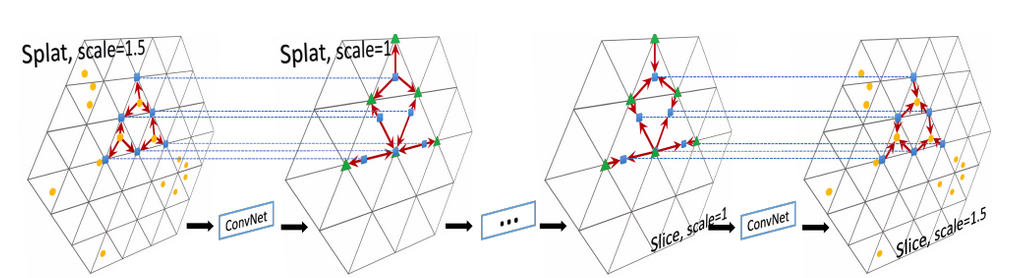
\includegraphics[width=1\linewidth]{latex/flow.png}
\end{center}
   \caption{Pipeline of HPLFlowNet\cite{hplf}.Hierarchical DownBCLs(Downsampling Bilateral Convolutional Layers) and UpBCLs(Upsampling Bilateral Convolutional Layers) on permutohedral lattice.}
\label{fig:flow}
\end{figure}

\subsection{Multi-layer Range Images Model}
At present, most of the input based on the projection method is a range image, but this has an obvious shortcoming. The point cloud on the same ray will be projected on the same pixel, because only one pixel can be stored  Point (usually save the nearest point), the information of the distant point is discarded.  This means that when reprojecting (projecting a range image to a three-dimensional point cloud), point clouds that are not involved in the calculation in the distance will be given the category label of the point cloud at the same pixel position.

\begin{figure}[pt]
\begin{center}
% \fbox{\rule{0pt}{2in} \rule{0.9\linewidth}{0pt}}
   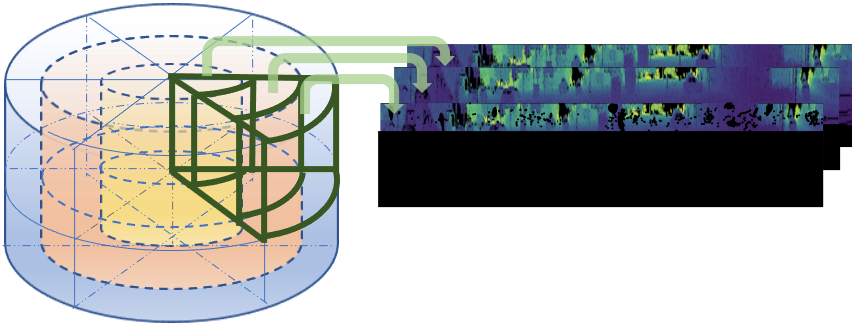
\includegraphics[width=1\linewidth]{latex/pro-vox.png}
\end{center}
   \caption{Multi-layer range images model: fusion of projection-based and voxel-based frameworks.}
\label{fig:provox}
\end{figure}
Inspired by Cylinder3D\cite{cylinder}, they converted the LiDAR point cloud into a cylindrical voxel representation. Considering the distribution nature of the LiDAR point cloud, the voxel size of the point cloud gradually increases from near to far, and the number of voxels gradually decreases, such as shown in Figure \ref{fig:provox}.  We thought that we could make a spherical projection of the voxel of each cylinder, so that we could solve the problem of point cloud projection overlap.  We propose a multi-layer distance image model, which performs multi-layer projection according to the distribution of point clouds in the distance direction.  As shown in the right part of Figure 6, the set of pixels of a certain size on each layer of image can be regarded as squashed voxels.  Through this model we can improve the recognition rate of distant objects.  The experimental part of Chapter 6 also verifies the feasibility of this model.

%-------------------------------------------------------------------------
\begin{figure*}[pt]
\centering
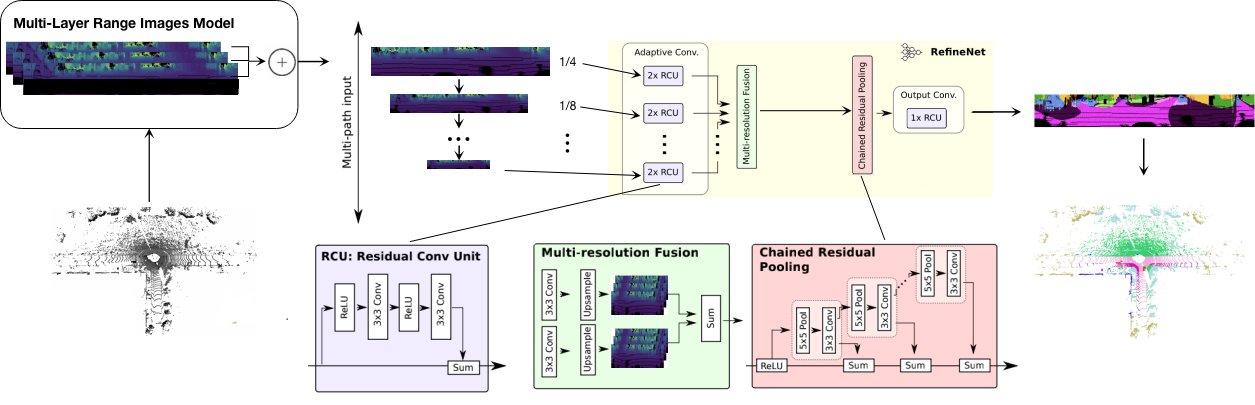
\includegraphics[width=1\linewidth,height=3in]{latex/framwork.png}
\caption{The overall framework of the algorithm MLRSeg which contains original point cloud, multi-layer distance image model, the individual components of our refinement network architecture RefineNet, semantic image map and semantic point cloud. Components in RefineNet employ residual connections with identity mappings. In this way, gradients can be directly propagated within RefineNet via local residual connections, and also directly propagate to the input paths via long-range residual connections, and thus we achieve effective end-to-end training of the whole system}
\label{fig:framework}
\end{figure*}

\subsection{Network Structure}
Generally, projection-based methods will use CNN. Due to the use of convolution or pooling layers, the image resolution is reduced. For this reason, Lin et al. proposed RefineNet\cite{12}, a multi-path enhanced network, which can segment the detailed structure in the image. Therefore, we have adopted RefineNet as the backbone of the network. RefineNet explicitly utilizes all the information of the downsampling process and uses remote residual connections to achieve high-resolution predictions.  At this time, the perfect features of the shallow layer can be directly used to strengthen the high-level semantic features.
The residual convolution module(RCU) contains activation and convolution operations, and then uses sum to fuse the feature maps before and after, which is the same in design in ResNet\cite{2016Deep}.  After the multi-resolution fusion module inputs the feature maps of the previous multiple resolutions into the fusion module, it first uses the convolutional layer to obtain the feature maps with the same size; then uses the upsampling operation to expand all the feature maps to new features of the same size  Figure; Finally, use the Sum operation to fuse all feature maps.  The purpose of chain residual is to capture contextual information from a large background area. Multiple pooling windows can obtain effective features and use the learned weights for fusion.

\subsection{Data collection}
For outdoor scenes and applications such as autonomous driving, typical LiDAR sensors, such as Velodyne HDL-64E LiDAR, can scan about 64 × 3000 = 192, 000 points for each frame, covering an area of 160×160×20 meters. Processing point clouds at such scale efficiently or even in real time is far beyond the capability of PointNetbased methods. Hence, much of the recent work follows the method
based on spherical projection. Instead of processing 3D points directly, these methods first transform a 3D LiDAR point cloud into a 2D LiDAR image and use 2D ConvNets to segment the point cloud. At first, Velodyne’s VLP-16 sensor is used and carried by Jackal, a robot car. However the points are too sparse so at last we use Rs-ruby by Robosense.\\
Rs-ruby is a 128 beam LIDAR specially designed for L4+ autonomous driving. Compared with rs- LIDAR--32,rs- ruby has3 times higher vertical angular resolution of0.1°, and maximum detection range improved by 2 to 3 times. Rs-ruby fully fulfills the requirements of high speed autonomous driving.Rs-ruby meets the requirement on low working emperature down to-30c, and has achieved breakthrough in anti-interference Resist interference of other LIDAR and ambient light in
all-weather.
\begin{figure}[p]
\centering
\subfigure[velodyne-16]{
\begin{minipage}[t]{0.5\linewidth}
\centering
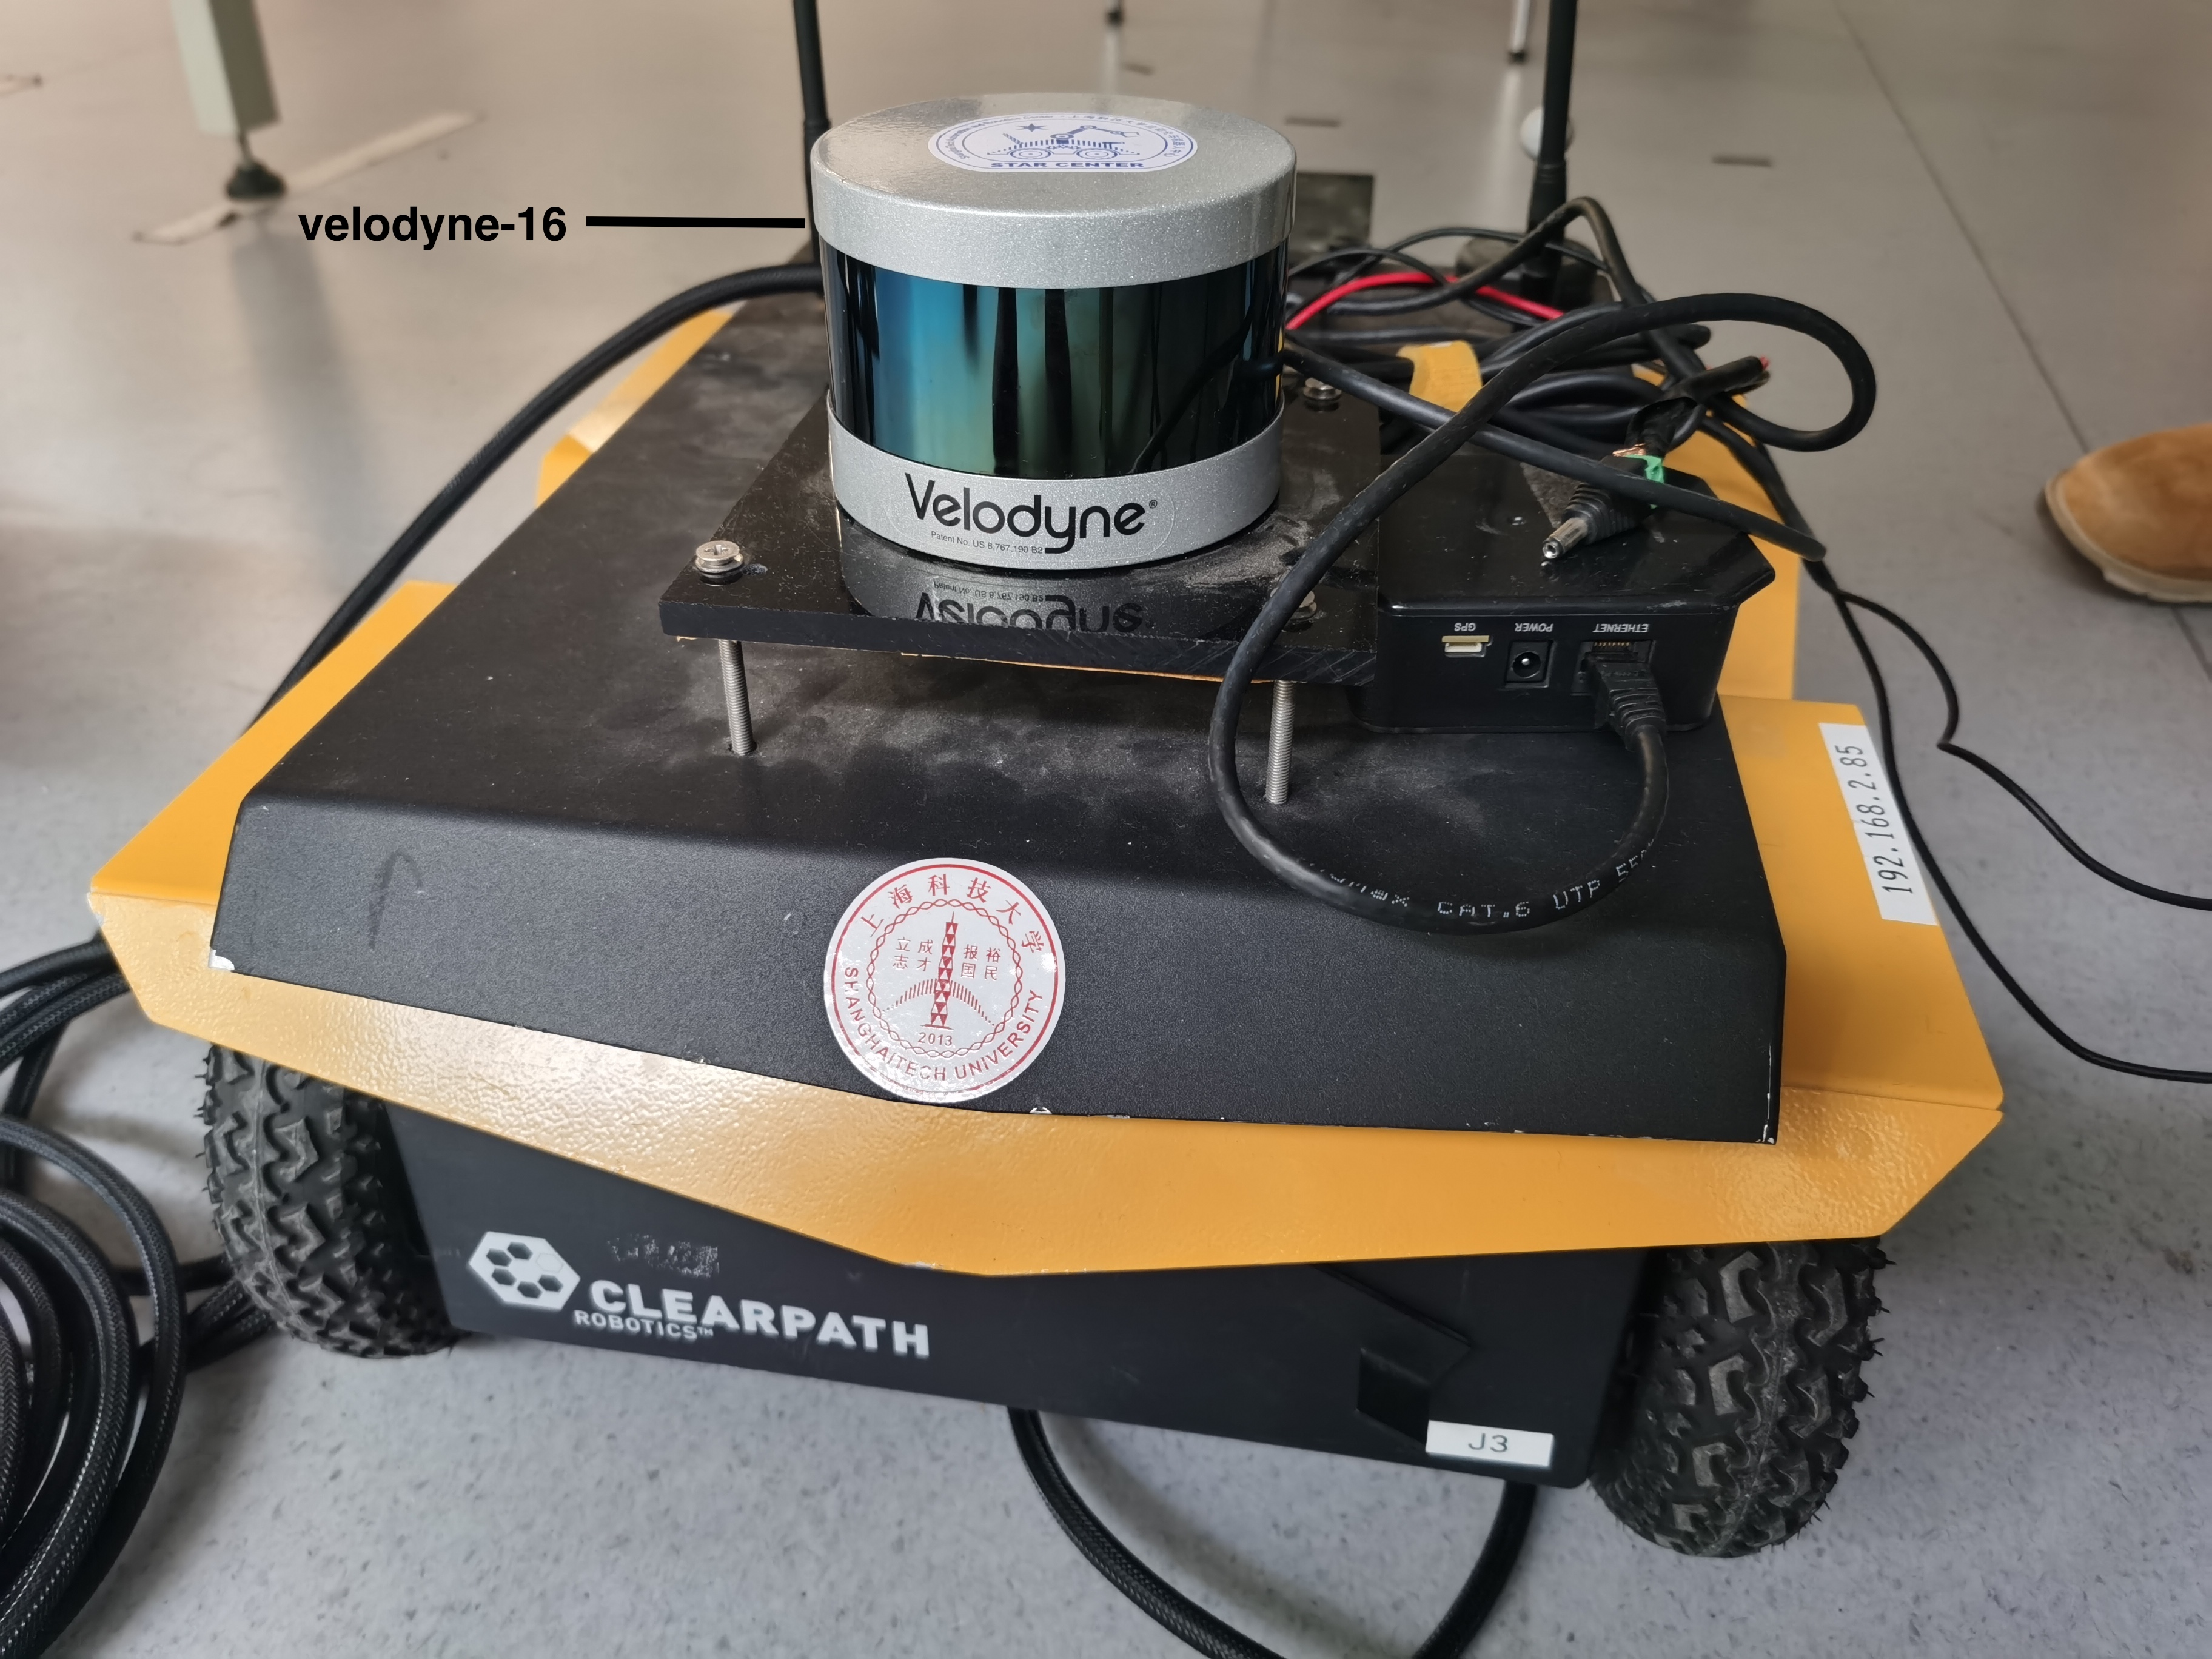
\includegraphics[height=1.3in]{latex/velodyne.jpg}
%\caption{fig1}
\end{minipage}%
}%
\subfigure[Robosense 128 beams]{
\begin{minipage}[t]{0.5\linewidth}
\centering
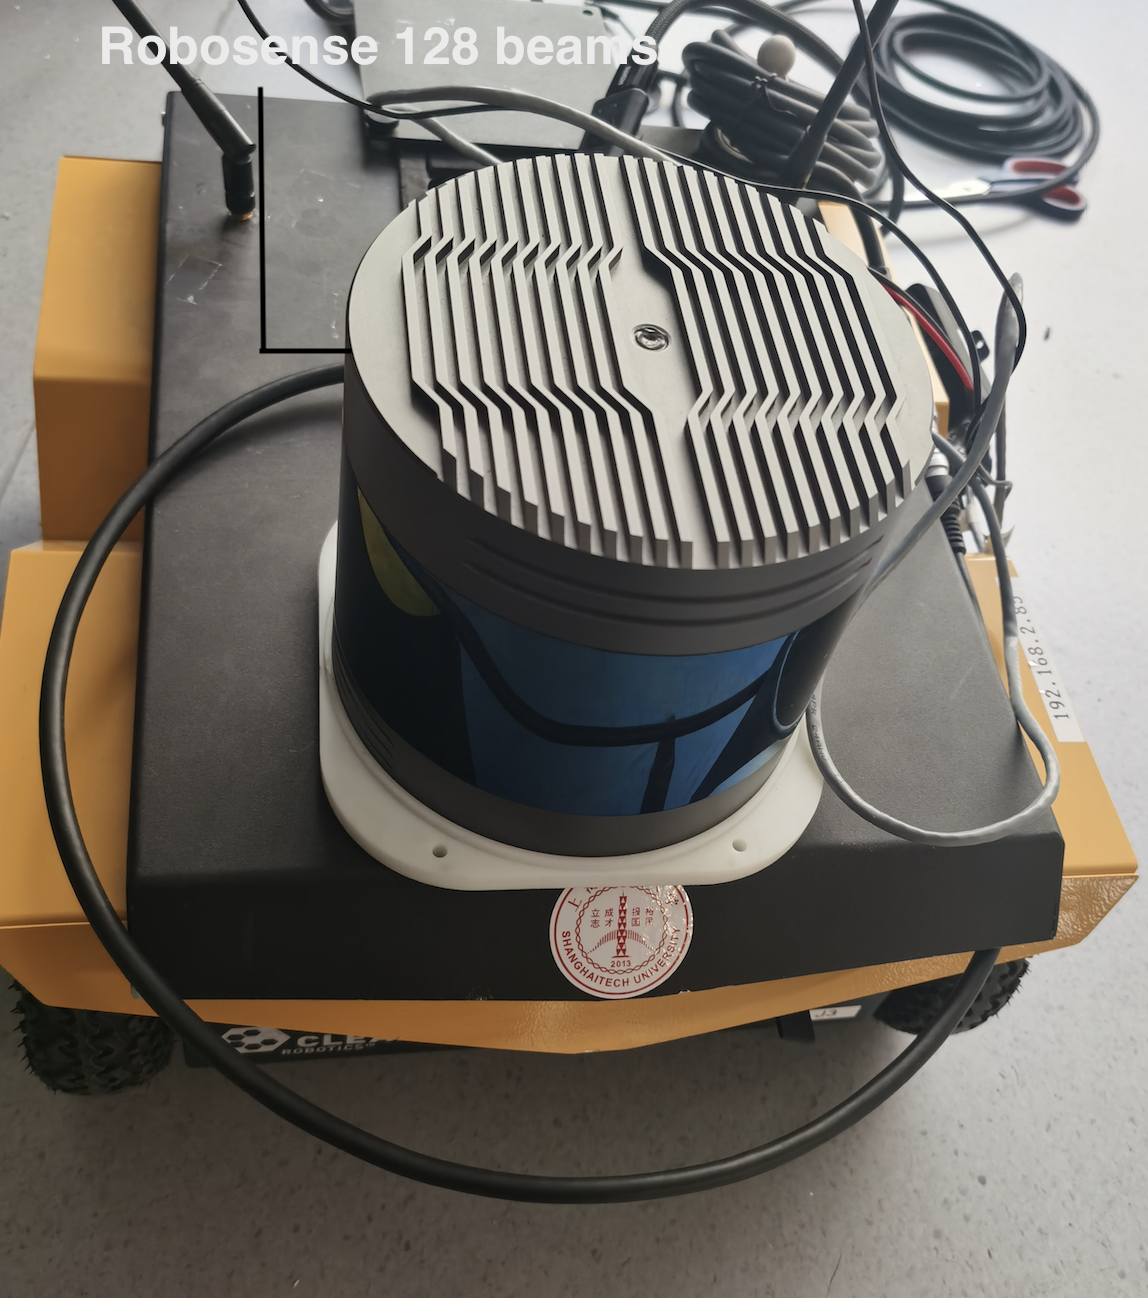
\includegraphics[height=1.3in]{latex/Robosense.png}
%\caption{fig2}
\end{minipage}%
}%
\centering
\caption{Jackal with velodyne-16 and Robosense}
\end{figure}
The pipeline figure shows that how to transform a raw point cloud data into data that can be imported as squeeze input.

% for pipeline part
\begin{figure*}[h]
\centering
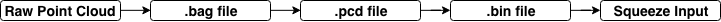
\includegraphics[width=1\linewidth]{robot pipeline.png}
\caption{Bag:This page describes the ROS bag format, which is a logging format for storing ROS messages in files. Files using this format are called bags, and have the file extension .bag. Bags are recorded, played back, and generally manipulated by tools in the rosbag and rqt_bag packages.
PCD files: The PCD (Point Cloud Data) is a file format for storing 3D point cloud data. It was created because existing formats did not support some of the features provided by the PCL library. PCD is the primary data format in PCL, but the library also offers the ability to save and load data in other formats (such as PLY, IFS, VTK, STL, OBJ, X3D). However, these other formats do not have the flexibility and speed of PCD files. One of the PCD advantages is the ability to store and process organized point cloud datasets. Another is very fast saving and loading of points that are stored in binary form.
\textbf{Binary file: Binary file contains the text of the document but also contain formatting information in binary form. Here, we use binary file to store numpy array containing our point cloud information.}
}\end{figure*}

\begin{figure*}[h]
\centering
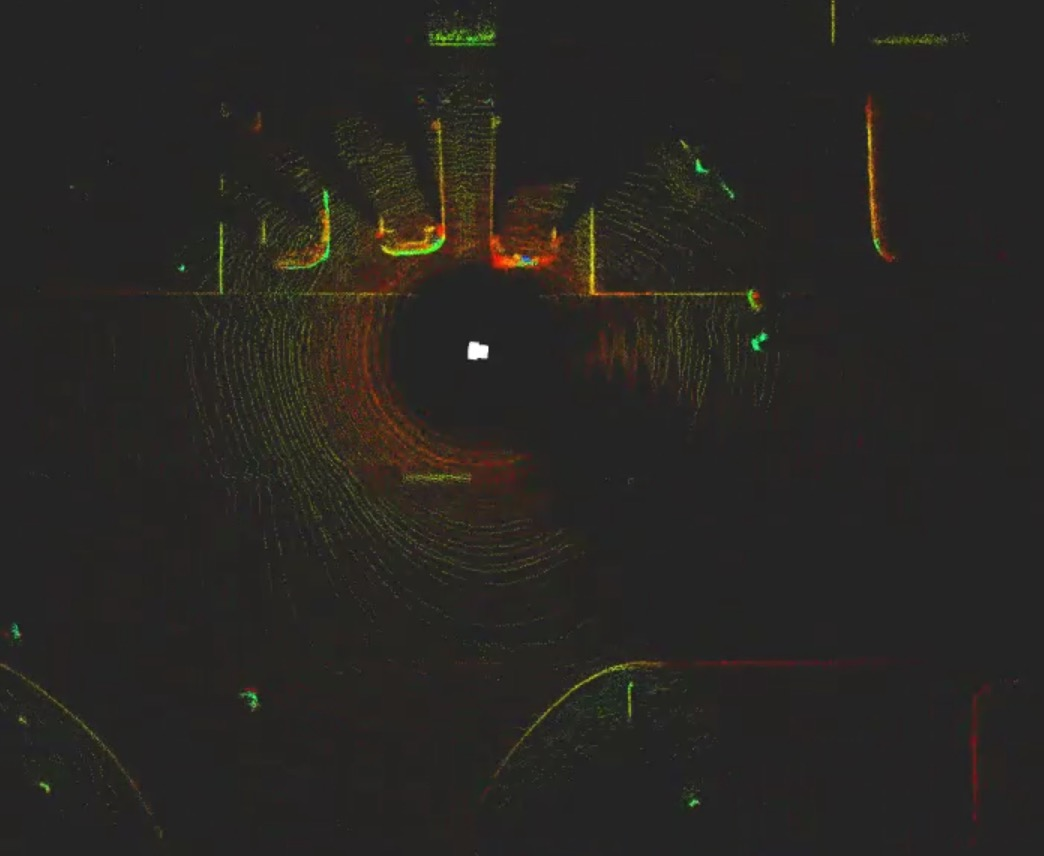
\includegraphics[width=1\linewidth]{latex/pc.jpg}
\caption{Point Cloud}
\end{figure*}

\section{Experiments(System Evaluation)}
The evaluation of the system is divided into two parts: qualitative and quantitative evaluation. The qualitative evaluation will use our scanned 3D point cloud of the ShanghaiTech University campus to visualize the effect. Quantitative evaluation will be performed on the SemanticKITTI dataset. After using our algorithm to predict the validation set, we will submit our results to SemanticKITTI’s semantic segmentation competition to obtain mean Jaccard or so-called intersection-over-union (mIoU)) over all classes, accuracy. We compare the recognition accuracy of different categories, overall accuracy (running time, memory consumption) with SqueezeSegV3\cite{xu2020squeezesegv3} with the best performing of the current projection-based methods 
\subsection{Fusion of Point-Projection framework}
In this project, we first considered the combination of the point-based method and the projection-based method, so we tried the SqueezeSegV3\cite{xu2020squeezesegv3} and RandLA\cite{2019RandLA} feature fusion algorithm. We input the feature map generated by  SqueezeSegV3\cite{xu2020squeezesegv3} into the RandLA\cite{2019RandLA} network as a prior feature map. In the process again, we need to consider the size of the feature and this is not an end-to-end algorithm.  Since the distance picture has a fixed size, but the points of the point cloud are disordered, this fusion needs further improvement.
Currently our algorithm has achieved initial progress, point and projection model accuracy and benefiting all above The algorithm has achieved excellent performance. As shown in Tabel \ref{tab:res}, the effect on people, motorcycles, bicycles and other small objects that are easy to recognize errors has also been improved.  However, the direct connection operation of this kind of network is too rough, accompanied by a long processing process, which is not suitable for the field of automatic driving that requires real-time data processing.
\begin{table*}[t] %h表示三线表在当前位置插入
%\setlength{\abovecaptionskip}{0.05cm} %设置三线表标题与第一条线间距
\tiny
\renewcommand\tabcolsep{0.5pt}
\centering
\caption{\textbf{The results comparison}} 
%表头文本加黑,但不加黑Table 1.字样,引入包即可:\usepackage[labelfont=bf]{caption}
\begin{tabular*}{\hsize}{@{\extracolsep{\fill}}ccccccccccccccccccccccccccccc} %{\hsize}使三线表自适应宽度,c表示文本居中
	\hline
 	%methods&accurancy&mIoU& {car}& {bicycle}& {motorcycle}& {truck}& {other-vehicle}& {person}& {bicyclist}& {road}& {parking}& {sidewalk}& {other-ground&building}& {fence}& {vegetation}& {trunk}& {terrain}& {pole}& {traffic-sign}\\
	\hline 
	SqueezeSeg53&0.891&0.527&0.861&0.309&0.478&0.507&\textbf{0.424}&0.522&0.524&\textbf{0.945}&0.473&\textbf{0.816}&0.003&0.802&0.472&0.825&0.525&0.720&0.424&0.382&\\
	RandLA &0.899&0.539&\textbf{0.942}&0.260&0.258&0.401&0.389&0.492&0.482&0.907&0.603&0.737&0.204&\textbf{0.869}&\textbf{0.563}&0.814&\textbf{0.613}&0.668&0.492&\textbf{0.477}\\
	Ours1& \textbf{0.903}&\textbf{0.543}&0.928&\textbf{0.363}& \textbf{0.5108}&0.318&0.365&\textbf{0.553}&\textbf{0.627}&0.934&0.390&0.800&0.366&0.858&0.421&\textbf{0.867}&0.588&\textbf{0.744}&\textbf{0.584}&0.422 \\
	Ours\_mul &0.885&0.504&0.862&0.220&0.469&0.377&0.388&0.383&0.474&0.9445&0.479&0.808&0.006&0.807&0.523&0.809&0.504&0.692&0.419&0.313\\
	MRL&0.883&0.505&0.888&0.160&0.327&0.666&0.314&0.525&0.566&0.000&0.914&0.326&0.766&0.863&0.460&0.825&0.507&0.695&0.457&0.312\\
	RefineNet&0.880&0.516&0.833&0.259&0.346&\textbf{0.795}&0.303&0.527&0.587&0.000&\textbf{0.936}&0.353&\textbf{0.797}&0.810&0.457&0.812&0.522&0.687&0.404&0.375\\
	\hline
	\label{tab:res}
\end{tabular*}
\end{table*}
\subsection{Performance of MLRSeg w.r.t. State-of-the-art}
The second experiment is designed to support our claim that our approach over-performs the state of the art in the task of scene semantic segmentation of 3D point clouds. Table \ref{tab:res} shows the difference between our RefineNet backbones 53layers and 7 other baseline  methods. Due to our limited computing resources, the batch size of our algorithm is 4, while the default size of SqueezeSeg is 8.
that this model can be a good proxy for the actual distance the remote the points are in the image. 

\subsection{Ablation Studies}
Tabel \ref{tab:res} also shows the influence of Multi-layer Range Images Model. We can see, from the experimental results of adding and not adding the model in Table \ref{tab:res}, our model has greatly improved the recognition of distant objects, and can supplement the information of objects with densely distributed light directions.  The current multi-layer model only provides more feature information for the first layer of pictures, and the points on other layers are not involved in direct prediction. However, due to the limitation of our computing resources, it is impossible to calculate the corresponding label for each layer of distance image, and give the weight according to the distance. Therefore, the mIou of our algorithm in Table \ref{tab:res} is lower than that of the existing algorithm. This phenomenon can be explained in this way. Once the weight of the distant object is larger, the probability of the close object being classified into the wrong category is greater, and our final classification is based on the point of the first layer of the image (near point)  This will lead to a decrease in the mIou.

%-------------------------------------------------------------------------
\section{Manual}
Our code will be uploaded to gitlab in the folder named MLRSeg. The instructions are tested on Ubuntu 16.04 with python 3.6 and Pytorch which the version corresponding to the GPU. The user's dataset needs to be stored according to the structure of Figure \ref{fig:fil}.
\begin{figure}
\begin{center}
% \fbox{\rule{0pt}{2in} \rule{0.9\linewidth}{0pt}}
   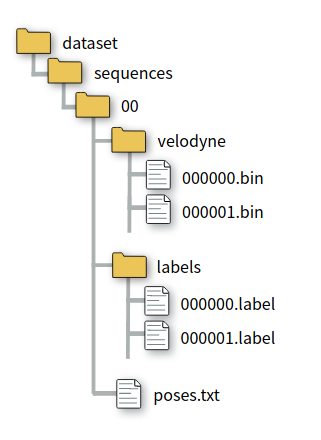
\includegraphics[width=0.6\linewidth,height=0.8\linewidth]{latex/file.png}
\end{center}
   \caption{The structure of dataset file system.}
\label{fig:fil}
\end{figure}
\lstset{language=bash, %用于设置语言为bash
	keywordstyle=\color{blue!70}\bfseries, %设置关键词为蓝色,需要引xcolor宏包
	basicstyle=\small,
	commentstyle=\ttfamily, %基本和注释的字体都使用默认的等宽,而非texlive调用的中文字体
	showstringspaces=false, %不显示中间的空格
}
\begin{itemize}
    \item Use pip to install required Python packages.
\end{itemize}
\begin{lstlisting}
pip install -r requirements.txt
\end{lstlisting}
\begin{itemize}
    \item We provide a demo script, you can find the prediction .label files and projected map in \./src/sample\_output file.
\end{itemize}
\begin{lstlisting}
cd ./src/tasks/semantic/
python demo.py -m /path/to/model
\end{lstlisting}
\begin{itemize}
    \item To infer the predictions for the entire dataset:
\end{itemize}
\begin{lstlisting}
cd ./src/tasks/semantic/
python infer.py -d /path/to/dataset/ 
-l /path/for/predictions -m /path/to/model
\end{lstlisting}
\begin{itemize}
    \item To infer the predictions for the entire dataset:
\end{itemize}
\begin{lstlisting}
python visualize.py -d /path/to/dataset/ 
-p /path/to/predictions/ -s SQ_Number
\end{lstlisting}
\begin{itemize}
    \item To train a network (from scratch):
\end{itemize}
\begin{lstlisting}
cd ./src/tasks/semantic/
python train.py -d /path/to/dataset 
-ac /config/arch/CHOICE.yaml 
-l /path/to/log
\end{lstlisting}
\begin{itemize}
    \item To train a network (from pretrained model):
\end{itemize}
\begin{lstlisting}
python train.py -d /path/to/dataset 
-ac /config/arch/CHOICE.yaml 
-l /path/to/log -p /path/to/pretrained
\end{lstlisting}
\begin{itemize}
    \item We can monitor the training process using tensorboard.
\end{itemize}
\begin{lstlisting}
tensorboard --logdir /file_path/
\end{lstlisting}


\section{Conclusions}
In this project, we proposed a U-Net-based network structure RefineNet with a multi-layer distance image model, created our own (ShanghaiTech campus) data set, and performed our algorithm MRLSeg from both qualitative and quantitative aspects.  The evaluation verifies the conclusion that our network can integrate features based on multiple methods, and can significantly improve the segmentation effect of small objects, densely distributed objects, and distant objects.  We also conducted performance analysis for the problems found in the experiment.  In the future, we will step by step to solve the optimization problems of the currently discovered quantization strategy and the optimization of the multi-layer distance image model expression, and supplement the experiments on time and computing resources.

\appendix  
\section{Multi-layer range images model}
\lstset{language=python, %用于设置语言为bash
	keywordstyle=\color{blue!70}\bfseries, %设置关键词为蓝色,需要引xcolor宏包
	basicstyle=\small,
	commentstyle=\ttfamily, %基本和注释的字体都使用默认的等宽,而非texlive调用的中文字体
	showstringspaces=false, %不显示中间的空格
	frame=shadowbox,  %边框
}
\begin{lstlisting}
if i==0:
d_s=0
else:
d_s=depth_max/(self.layer_num+1-i)

d=depth[depth>=d_s]
#print(proj_x.shape)
proj_x = proj_x[depth>=d_s]
# round and clamp for use as index
proj_x = np.floor(proj_x)
proj_x = np.minimum(self.proj_W-1, proj_x)
proj_x = np.maximum(0,
 proj_x).astype(np.int32)
if i==0:
self.proj_x =np.copy(proj_x)

proj_y = proj_y[depth>=d_s]
proj_y = np.floor(proj_y)
proj_y = np.minimum(self.proj_H - 1, proj_y)
proj_y = np.maximum(0, proj_y)
.astype(np.int32)
if i==0:
self.proj_y = np.copy(proj_y)

# order in decreasing depth
indices = np.arange(d.shape[0])
order = np.argsort(d)[::-1]
depth = d[order]
indices = indices[order]
points = self.points[order]
remission = self.remissions[order]
proj_y = proj_y[order]
proj_x = proj_x[order]
# assing to images
self.proj_range[i,proj_y\
, proj_x] = depth
self.proj_xyz[i,proj_y,\
proj_x] = points
self.proj_remission[i,proj_y,proj_x]\
=remission
self.proj_idx[i,proj_y, proj_x] = indices
self.proj_mask = (self.proj_idx> 0)\
.astype(np.int32)
\end{lstlisting}
\begin{lstlisting}
proj = torch.cat([proj_range.\
unsqueeze(0).clone(),
proj_xyz.clone().permute(3,0,1,2),
proj_remission.unsqueeze(0).clone()])
#proj_remission.unsqueeze(0).clone()])
proj=proj.reshape(proj.shape[0]* \
proj.shape[1,proj.shape[2],proj.shape[3])
sensor_img_means=[]
sensor_img_stds=[]

sensor_img_means=self.sensor_img_means.\
repeat(scan.layer_num)
sensor_img_stds=self.sensor_img_stds.\
repeat(scan.layer_num)
#sensor_img_stds=self.sensor_img_stds.\
repeat(scan.layer_num)
proj = (proj - sensor_img_means[:,None,None]) / \
sensor_img_stds[:,None,None]
proj = proj * proj_mask.float()
\end{lstlisting}
\section{Backbone of Network}
\begin{lstlisting}
class BasicBlock(nn.Module):
expansion = 1

def __init__(self, inplanes, planes, \
stride=1, downsample=None):
super(BasicBlock, self).__init__()
self.conv1 = conv3x3(inplanes, 
             planes, stride)
self.bn1 = nn.BatchNorm2d(planes)
self.relu = nn.ReLU(inplace=True)
self.conv2 = conv3x3(planes, planes)
self.bn2 = nn.BatchNorm2d(planes)
self.downsample = downsample
self.stride = stride

def forward(self, x):
residual = x

out = self.conv1(x)
out = self.bn1(out)
out = self.relu(out)

out = self.conv2(out)
out = self.bn2(out)

if self.downsample is not None:
residual = self.downsample(x)

out += residual
out = self.relu(out)

return out


class Bottleneck(nn.Module):
expansion = 4

def __init__(self, \
inplanes, planes, stride=1, downsample=None):
super(Bottleneck, self).__init__()
self.conv1 = nn.Conv2d(inplanes, planes, 
             kernel_size=1, bias=False)
self.bn1 = nn.BatchNorm2d(planes)
self.conv2 = nn.Conv2d(planes, planes,
             kernel_size=3, stride=stride, 
             padding=1, bias=False
)
self.bn2 = nn.BatchNorm2d(planes)
self.conv3 = nn.Conv2d(planes, planes * 4,
            kernel_size=1, bias=False)
self.bn3 = nn.BatchNorm2d(planes * 4)
self.relu = nn.ReLU(inplace=True)
self.downsample = downsample
self.stride = stride

def forward(self, x):
residual = x

out = self.conv1(x)
out = self.bn1(out)
out = self.relu(out)

out = self.conv2(out)
out = self.bn2(out)
out = self.relu(out)

out = self.conv3(out)
out = self.bn3(out)

if self.downsample is not None:
residual = self.downsample(x)

out += residual
out = self.relu(out)

return out


class Backbone(nn.Module):
def __init__(self, params, num_classes=21):
self.inplanes = 64
super(Backbone, self).__init__()
self.use_range =\
params["input_depth"]["range"]
self.use_xyz =\
params["input_depth"]["xyz"]
self.use_remission =\
params["input_depth"]["remission"]
self.drop_prob = params["dropout"]
self.bn_d = params["bn_d"]
self.OS = params["OS"]
self.layers = params["extra"]["layers"]
print("Using Refinenet"
+ str(self.layers) + " Backbone")
print("num_classes",num_classes)

# input depth calc
self.input_depth = 0
self.input_idxs = []
if self.use_range:
self.input_depth += 1
self.input_idxs.append(0)
if self.use_xyz:
self.input_depth += 3
self.input_idxs.extend([1, 2, 3])
if self.use_remission:
self.input_depth += 1
self.input_idxs.append(4)
print("Depth of backbone input = ",
self.input_depth)

layers=[3, 4, 6, 3]

self.do = nn.Dropout(p=0.5)
self.conv1 = nn.Conv2d(self.input_depth, 64, 
kernel_size=3, stride=1,
padding=1, bias=False)
self.bn1 = nn.BatchNorm2d(64)
self.relu = nn.ReLU(inplace=True)
self.maxpool = nn.MaxPool2d(kernel_size=3,
stride=2, padding=1)
self.layer1 = self._make_layer(Bottleneck,
            64, layers[0])
self.layer2 = self._make_layer(Bottleneck, 
            128, layers[1], stride=2)
self.layer3 = self._make_layer(Bottleneck, 
            256, layers[2], stride=2)
self.layer4 = self._make_layer(Bottleneck, 
            512, layers[3], stride=2)
self.p_ims1d2_outl1_dimred = conv1x1(2048, 
            512, bias=False)
self.mflow_conv_g1_pool =\
self._make_crp(512, 512, 4)
self.mflow_conv_g1_b3_joint_varout_dimred =\ 
conv1x1(512, 256, bias=False)
self.p_ims1d2_outl2_dimred =\
conv1x1(1024, 256, bias=False)
self.adapt_stage2_b2_joint_varout_dimred =\ 
conv1x1(256, 256, bias=False)
self.mflow_conv_g2_pool =\
self._make_crp(256, 256, 4)
self.mflow_conv_g2_b3_joint_varout_dimred =\ 
conv1x1(256, 256, bias=False)

self.p_ims1d2_outl3_dimred =\
conv1x1(512, 256, bias=False)
self.adapt_stage3_b2_joint_varout_dimred =\
conv1x1(256, 256, bias=False)
self.mflow_conv_g3_pool =\
self._make_crp(256, 256, 4)
self.mflow_conv_g3_b3_joint_varout_dimred =\ 
conv1x1(256, 256, bias=False)

self.p_ims1d2_outl4_dimred =\
conv1x1(256, 256, bias=False)
self.adapt_stage4_b2_joint_varout_dimred =\
conv1x1(256, 256, bias=False)
self.mflow_conv_g4_pool =\
self._make_crp(256, 256, 4)

self.clf_conv = nn.Conv2d(
256, num_classes, kernel_size=3, 
stride=1, padding=1, bias=True
)

def _make_crp(self, in_planes,
out_planes, stages):
layers = [CRPBlock(in_planes,
out_planes, stages)]
return nn.Sequential(*layers)

def _make_layer(self, block, planes,
blocks, stride=1):
downsample = None
if stride != 1 or self.inplanes != \
planes * block.expansion:
downsample = nn.Sequential(
nn.Conv2d(
self.inplanes,
planes * block.expansion,
kernel_size=1,
stride=stride,
bias=False,
),
nn.BatchNorm2d(planes * block.expansion),
)

layers = []
layers.append(block(self.inplanes, planes,
stride, downsample))
self.inplanes = planes * block.expansion
for i in range(1, blocks):
layers.append(block(self.inplanes, planes))

return nn.Sequential(*layers)

def forward(self, x):
# filter input
x = x[:, self.input_idxs]
x = self.conv1(x)
x = self.bn1(x)
x = self.relu(x)
   # x = self.maxpool(x)

l1 = self.layer1(x)
l2 = self.layer2(l1)
l3 = self.layer3(l2)
l4 = self.layer4(l3)

l4 = self.do(l4)
l3 = self.do(l3)

x4 = self.p_ims1d2_outl1_dimred(l4)
x4 = self.relu(x4)
x4 = self.mflow_conv_g1_pool(x4)
x4 = self.mflow_conv_g1_b3_joint\
_varout_dimred(x4)
x4 = nn.Upsample(size=l3.size()[2:],
mode="bilinear", align_corners=True)(x4)

x3 = self.p_ims1d2_outl2_dimred(l3)
x3 = self.adapt_stage2_b2_joint\
_varout_dimred(x3)
x3 = x3 + x4
x3 = F.relu(x3)
x3 = self.mflow_conv_g2_pool(x3)
x3 = self.mflow_conv_g2_b3_joint\
_varout_dimred(x3)
x3 = nn.Upsample(size=l2.size()[2:],
mode="bilinear", align_corners=True)(x3)

x2 = self.p_ims1d2_outl3_dimred(l2)
x2 = self.adapt_stage3_b2_joint\
_varout_dimred(x2)
x2 = x2 + x3
x2 = F.relu(x2)
x2 = self.mflow_conv_g3_pool(x2)
x2 = self.mflow_conv_g3_b3_joint\
_varout_dimred(x2)
x2 = nn.Upsample(size=l1.size()[2:],
mode="bilinear", align_corners=True)(x2)

x1 = self.p_ims1d2_outl4_dimred(l1)
x1 = self.adapt_stage4_b2_joint\
_varout_dimred(x1)
x1 = x1 + x2
x1 = F.relu(x1)
x1 = self.mflow_conv_g4_pool(x1)
# print(x.shape)
# print(l1.shape,l2.shape,l3.shape,l4.shape)
# print(x1.shape,x2.shape,x3.shape,x4.shape)


out = self.clf_conv(x1)
out = F.softmax(out,dim=1)
return out

def get_input_depth(self):
return self.input_depth
\end{lstlisting}  
\label{app:A}

{\small
\bibliographystyle{ieee_fullname}
\bibliography{egbib}
}

\end{document}
